\documentclass[12pt,a4paper,notitlepage]{report}

\usepackage[polish, english]{babel}
\usepackage[T1]{fontenc}
\usepackage[utf8]{inputenc}
\usepackage[top=2.5cm, bottom=2.5cm, left=3.5cm, right=3.5cm]{geometry}
\usepackage{graphicx} 
\usepackage{subcaption}
\usepackage{wrapfig}

\makeatletter

\renewcommand{\maketitle}{\begin{titlepage}

    \begin{center}
    \LARGE Uniwersytet Przyrodniczy we Wroc\l{}awiu\\
    \Large Wydzia\l{} Biologii i Hodowli Zwierz\k{a}t\\
    \large Kierunek: Bioinformatyka\\
    Studia stacjonarne drugiego stopnia\\
    Specjalno\'s\'c: Biostatystyka i programowanie bioinformatyczne
    \end{center}

    \vspace{3cm}

    \begin{center}
    \huge \@author \\
    \large 115962
    
    \vspace{2cm}
    
     \textbf{\Huge \@title}
     \end{center}

    \vspace{5cm}
    
    \begin{flushright}
     {\large Praca wykonana pod kierunkiem:}\\
         dr Anna Mucha\\
         Katedra Genetyki
     \end{flushright}

    \vspace*{\stretch{6}}

    \begin{center}
    \Large Wroc\l{}aw, 2020
    \end{center}

  \end{titlepage}%
}

\makeatother

\author{Aneta Sowi\'nska}
\title{Analysis of selected indicators for tonsillectomy}
\linespread{1.3}

\begin{document}

%---------------- Strona tytułowa -----------------

\maketitle

%------------------ Oświadczenie ------------------


\noindent Wroc\l{}aw, dnia ...............
\vspace{3cm}

\begin{flushleft}
\textbf{\textit{\large Oświadczenie opiekuna pracy}}
\end{flushleft}
Oświadczam, że niniejsza praca została przygotowana pod moim kierunkiem i stwierdzam, że spełnia ona warunki do przedstawienia jej w postępowaniu o nadanie tytułu zawodowego.
\vspace{2cm}
\begin{flushright}
Podpis opiekuna pracy……………………
\end{flushright}

\vspace{2cm}
\begin{flushleft}
\textbf{\textit{\large Oświadczenie opiekuna pracy}}
\end{flushleft}
Oświadczam, że niniejsza praca została przygotowana pod moim kierunkiem i stwierdzam, że spełnia ona warunki do przedstawienia jej w postępowaniu o nadanie tytułu zawodowego.
\vspace{2cm}
\begin{flushright}
Podpis autora pracy ..................................
\end{flushright}

%------------------- Abstrakt -------------------

\clearpage
\linespread{1.3}
\begin{abstract}
\vspace{0.5cm}
\begin{center}
\textbf{Analysis of selected indicators for tonsillectomy}
\end{center}
\vspace{0.5cm}
Lorem ipsum dolor sit amet, consetetur sadipscing elitr, sed diam nonumyeirmod tempor invidunt ut labore et dolore magna aliquyam erat, sed diamvoluptua. At vero eos et accusam et justo duo dolores et ea rebum. Stet clita kasd gubergren, no sea takimata sanctus est Lorem ipsum dolor sit amet.Lorem ipsum dolor sit amet, consetetur sadipscing elitr, sed diam nonumyeirmod tempor invidunt ut labore et dolore magna aliquyam erat, sed diamvoluptua. At vero eos et accusam et justo duo dolores et ea rebum. Stet clita kasd gubergren, no sea takimata sanctus est Lorem ipsum dolor sit amet.Lorem ipsum dolor sit amet, consetetur sadipscing elitr, sed diam nonumyeirmod tempor invidunt ut labore et dolore magna aliquyam erat, sed diamvoluptua. At vero eos et accusam et justo duo dolores et ea rebum. \\ \\
\textbf{Keywords:} tonsillectomy, halitosis, PCA.

\end{abstract}

%------------------ Spis treści -------------------

\tableofcontents


%-----------Pocztek części zasadniczej-----------

\clearpage
\linespread{1.3}
\chapter{Introduction}
Tu będzie napisane: \\
Czym  jest halitoza, przyczyny halitozy (substacje chemiczne, badania mikrobiologiczne, dieta, choroby układu pokarmowego, choroby układu oddechowego, schorzenia ogólnoustrojowe), diagnostyka haliotozy (badania subiektywne i obiektywne), leczenie halitozy, cel badawczy: czy istnieje związek między przewlekłym przerostowym zapaleniem migdałków podniebiennych a halitozą? Czy haliotoza może być predyktorem do przeprowadzenia zabiegu tonsillektomii? Jakie inne objawy mogą wpływać na halitozę?

%---Material and methods ----
\chapter{Material and methods}
\section{Material}

41 patients including 29 women and 13 men, ranging age from 18 to 56 years (mean 27.02, SD 7.86) with chronic hyperplastic tonsillitis and halitosis were qualified for tonsillectomy and therefore selected for the study. \mbox{A detailed} anamnesis was conducted by otolaryngologists and dentists, and microbiological tests were carried out in the laboratory of the Academic Clinical Hospital in Wroclaw. Also, routine laboratory tests and two surveys were conducted in order to eliminate causes of halitosis other than those indicative of tonsillitis. Patients answered questions related to their medical history, food habits, smoking cigarettes and oral hygiene. 
Those who confirmed the occurrence of any gastrointestinal, pulmonary or other systemic metabolic disorders in the survey were eliminated from the research group.
Another exclusion criteria included smokers, heavy alcoholic drinkers, improper oral hygiene and \textit{Helicobacter pylori} carriers. Dental examination excluded also patients with carious lesions, exposed tooth pulps, peridonthal diseases and thick tongue coat.

\section{Methods}

Patients underwent both subjective and objective evaluation of oral odor. 
For a subjective assessment of an unpleasant odor in the mouth each patient underwent organoleptic examination before tonsillectomy. Patients were neither allowed to take antibiotics for a period of three weeks, consume garlic, onion and spicy dishes for 24 hours nor apply perfume. Within 12 hours, it was also recommended to avoid food intake and drinks, brush teeth, use breath fresheners and smoke cigarettes. During the study, the smell of air exhaled through the mouth was compared with the smell of air exhaled through the nose (when mouth closed). The patient then exhaled into a transparent tube 10 cm long and 2.5 mm in diameter. In order to assess the intensity of the unpleasant smell from the mouth a six-grade Rosenberg \cite{Rosenberg92} scale was used which is the most widely used scale of halitosis. The odor was classified between 0 and 5, where: 0 - absence of odor, 1 - barely noticeable odor, 2 - slight malodor, 3 - moderate malodor, 4 - strong malodor and 5 - severe malodor.\

For objective assessment of halitosis each patient underwent a Man-hal-II Halimeter test as well. This sulfide monitor measures volatile sulfur compounds (VSCs) such as hydrogen sulfide, methyl mercaptan and dimethyl sulfide which are contributing factors for halitosis. Each sample was taken after 3 minute re-stabilization period when patients were breathing through the nose with  mouths kept closed. During the test the device's straw was inserted into the subject’s mouth and one was asked to exhale briefly for 30 seconds. 
The procedure was repeated in three trials for each patient and the peaks' values were recorded in parts per billion (ppb) sulfide equivalents \cite{Alasqah16}.
In order to obtain reliable results, patients could not eat, drink, smoke, chew gum, brush their teeth, use the brush, fresheners or oral hygiene products for 12 hours prior to the halimetric test. It was also recommended not to use cosmetics such as perfumes, aftershave or lipstick. \

Organoleptic and halimetric examination was repeated for each patient, at least 2-3 months after removal of the palatine tonsils and completion of the healing process.

The value of the average of the three measurements of VSC was used for further statistical analysis. Depending on the chosen criterion of division, two or three groups of patients have been distinguished. First one considered 100 ppb as threshold dividing group into normal (when below) and abnormal (when above the threshold). Second, more detailed criterion included intermediate states as follows: the range up to 100 ppb considered as correct, 100 - 180 ppb as a light form of disease and above 250 ppb as a severe one \cite{Lee04}. However, the study group did not include patients belonging to the latter (Fig. \ref{Fig_2.1}).  


\begin{figure}[h]
 
\begin{subfigure}{0.5\textwidth}
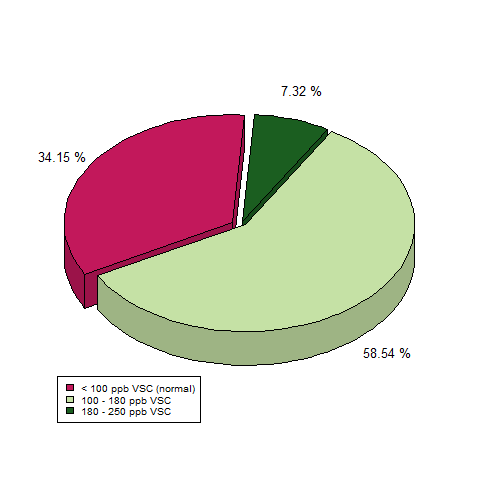
\includegraphics[width=1\linewidth, height=6cm]{./Figures/Fig_2.1a} 
\caption{the ratio of groups with different forms of the disease}
\label{Fig_2.1a}
\end{subfigure}
\begin{subfigure}{0.5\textwidth}
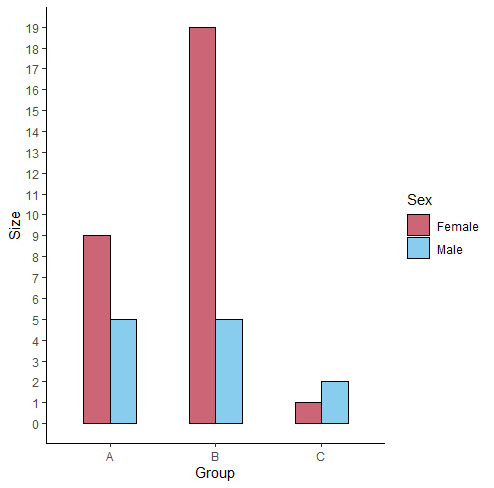
\includegraphics[width=1.1\linewidth, height=6cm]{./Figures/Fig_2.1b}
\caption{the gender distribution within groups A: < 100 ppb,  B: 100 - 180 ppb, C: > 180 ppb VSC}
\label{Fig_2.1b}
\end{subfigure}
 
\caption{Groups of patients due to the level of VSC before tonsillectomy.}
\label{Fig_2.1}
\end{figure}


Principal Component Analysis (PCA) was used in order to validate the above classification. This method enables finding the directions of maximum variance in high-dimensional data and project it onto a smaller dimensional subspace while retaining most of the information. In the following work script written in R programming language was used to perform the analysis. PCA was performed using \textit{FactoMineR} which is an R package dedicated to multivariate Exploratory Data Analysis, as well as \textit{factoextra} to extract and visualize the results. There are also other, built-in R functions avaliable - \textit{princomp()} and \textit{prcomp()}. The preceding one uses the spectral decomposition approach, while the functions \textit{prcomp()} and  \textit{FactoMineR::PCA()} use the singular value decomposition.

Comparisons between groups and within groups were made using appropriate statistical tests, after checking the assumptions authorizing to carry them out.
The gender distribution was included in each group. Considered level of significance for all of the statistical tests was 5\% (p < 0,05).



%----------- Results ------------
\chapter{Results}
\section{Comparison between groups}

\subsection{General statistics} 
\noindent
\begin{tabular}{lcccc}
\hline Feature 				& Female 	& Male 		& Total 		&  Comparison \\
 		 					& n = 29 	& n = 12	& n = 41	&  (\textit{p-value}) \\
\hline
\bf{Age}					&			&			&			&		\\
\indent mean				& 26.69		& 27.83		& 27.02		& 		\\
\indent sd					& 8.49		& 6.32		& 7.86		& 0.6391 \\
\indent me					& 24.00		& 27		& 25.00		& 		\\
\indent spread				& 18.00-56.00 & 19.00-36.00	& 18.00-56.00 & \\
\hline

\bf{Living place} 			&			&			&			&		\\
\indent village				& 5 (17.24)	& 0 (0.00)	& 5	(12.20)	& 		\\
\indent town					& 2 (6.90)	& 1	(8.33) 	& 3	(17.85) 	&  0.3078 \\
\indent city					& 22 (75.86)	& 11 (91.67) & 33 (80.49) & 		\\
\hline

\bf{Profession} 				&			&			&			&		\\
\indent school-age student	& 2 (6.90)	& 2 (16.67)	& 4	(9.76) 	& 		\\
\indent student				& 6 (20.69)	& 1	(8.33) 	& 7	(17.10) 	& 0.1834 \\
\indent blue-collar worker		& 3 (10.35)	& 4 (33.33) 	& 7 (17.10) 	& 		\\
\indent white-collar worker	& 18 (62.07)	& 5 (41.67) 	& 23 (56.10) & 		\\
\hline

\bf{Education} 				&			&			&			&		\\
\indent elementary			& 1 (3.45)	& 2 (16.70)	& 3	(7.32) 	& 		\\
\indent secondary			& 13 (44.80)	& 5	(41.70) 	& 18 (43.90) & 0.2699 \\
\indent higher				& 15 (51.70)	& 5 (41.70) 	& 20 (48.80) & 		\\
\hline

\end{tabular} \\ \\

The comparison of features: Age, Living place, Profession and Education between men and women was made with Student's t test (\textit{stats::t.test}) after checking the assumption of normality and homogeneity of variance. No statistically significant difference was observed in terms of analyzed features (p > 0.05).

\subsection{Halitometry results}
\noindent
\begin{tabular}{lcccc}
\hline VSC [ppb] 				& Female 	& Male 		& Total 		&  Comparison  \\
 		 					& n = 29 	& n = 12	& n = 41	&  (\textit{p-value}) \\
\hline
\bf{Before tonsillectomy}		&			&			&			&		\\
\indent mean				& 115.03	& 107.92	& 113.00	& 		\\
\indent sd					& 37.89		& 67.81		& 47.76		& 0.5378 \\
\indent me					& 120.00	& 105.00	& 117.00	& 		\\
\indent spread				& 22.00-186.00 & 25.00-238.00 & 22.00-238.00	 & \\
\hline

\bf{After tonsillectomy}		&			&			&			&		\\
\indent mean				& 43.52		& 45.08		& 43.98		& 		\\
\indent sd					& 19.20		& 24.81		& 20.66		& 0.8185 \\
\indent me					& 50.00		& 36.00		& 40.00 		& 		\\
\indent spread				& 7.00-80.00 & 23.00-113.00	& 7.00-113.00 & \\
\hline

\end{tabular} \\ \\

The comparison of measurement before tonsillectomy was made with Wilcoxon test (\textit{stats::wilcox.test}) due to heterogeneity of variance between groups (female vs male, \textit{p-value} = 0.01564). 

The comparison of VSC before and after tonsillectomy was made with Welch Two Sample t-test (\textit{stats::t.test} with paired=FALSE argument). According to p-value = 0.8471 we do have basis to accept the null hypothesis that the means in both groups are equal. 


\begin{figure}[h]
 
\begin{subfigure}{0.5\textwidth}
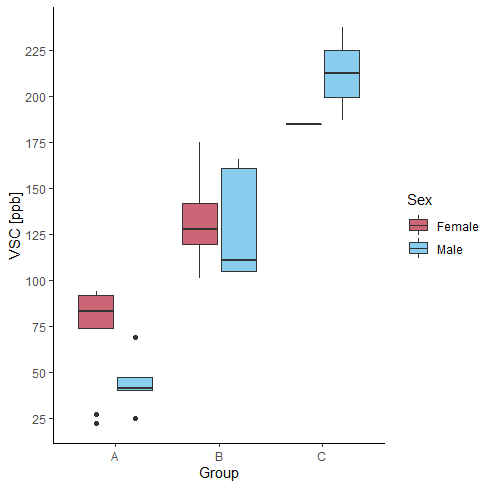
\includegraphics[width=1\linewidth, height=6cm]{./Figures/Fig_3.1a} 
\caption{before tonsillectomy}
\label{Fig_3.1a}
\end{subfigure}
\begin{subfigure}{0.5\textwidth}
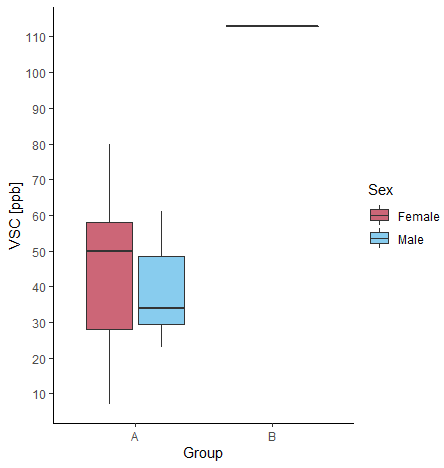
\includegraphics[width=1\linewidth, height=6cm]{./Figures/Fig_3.1b}
\caption{after tonsillectomy}
\label{Fig_3.1b}
\end{subfigure}
 
\caption{Levels of VSC in groups with split on gender. Groups A: < 100 ppb,  B: 100 - 180 ppb, C: > 180 ppb VSC}
\label{Fig_3.1}
\end{figure}

After tonsillectomy, there was only one patient with light form of halitosis - a 29-year old man with 113 ppb of VSC.
The avarage level of VSC dropped by 106.51 ppb.

\section{PCA results}


In order to determine the minimum number of principal components (PCs) that account for most of the variation in analyzed data two methods were used. The first one was based on the proportion of variance that the components explain. The acceptance level of variance was set to 80\%, thus PC3 might be taken as the cut-off point.

\begin{figure}[h]
	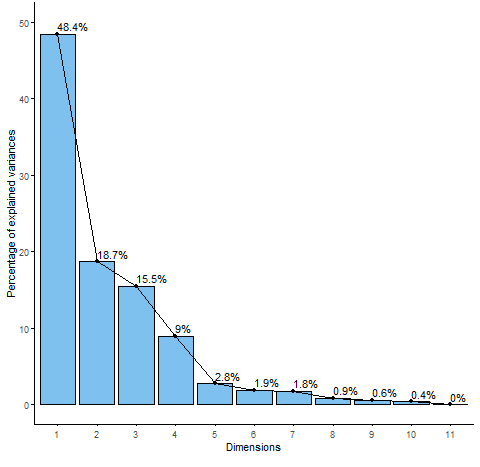
\includegraphics[scale=0.80]{./Figures/Fig_3.2}
	\caption{Eigenvalues.}
	\label{Fig_3.2}
\end{figure}	

\begin{wrapfigure}{l}{0.45\textwidth}
	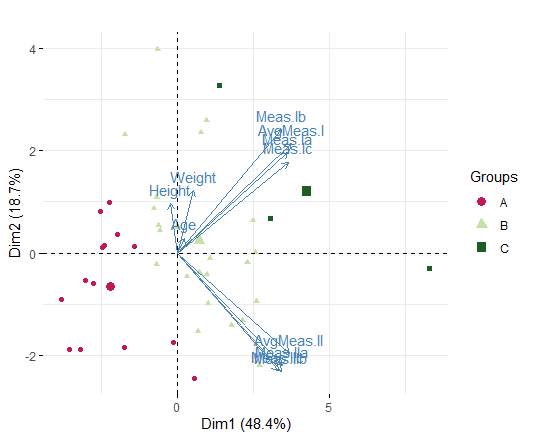
\includegraphics[scale=0.6]{./Figures/Fig_3.3}
	\caption{Scree plot.}
	\label{Fig_3.3}
\end{wrapfigure}	

An alternative method of estimating the number of principal components is the scree plot, which orders the eigenvalues in descending order. The number of PCs is selected at the point where there is a relative decrease in the amount of variance explained by given component. In that case, both methods indicate the same cut-off point which is PC3 meaning that first three principal components explain 82.61\% of the variation in the data.

Examining the magnitude and direction of the coefficients for the original variables allows to interpret each principal component. In these results, first and second principal component has positive associations with the average measurements of VSC (before and after tonsillectomy), so this component primarily measures surgery effectiveness. The second component has positive associations with individual measurements of VSC, so this component primarily measures repeatability of results. The third component has large positive associations with height and weight, so this component primarily measures the patient's body mass index. 

A PCA biplot (Fig. \ref{Fig_3.4}) shows both principal component scores of samples (here already grouped into three) and loadings of variables (so called loading plot). The further away vectors (variables) are from the origin, the more influence they have on that principal component.  From loading plots we can notice how well are the variables correlated with each other: a small angle implies positive correlation, a large one suggests negative correlation. A right angle indicates no correlation between two features.

\begin{figure}[h]
	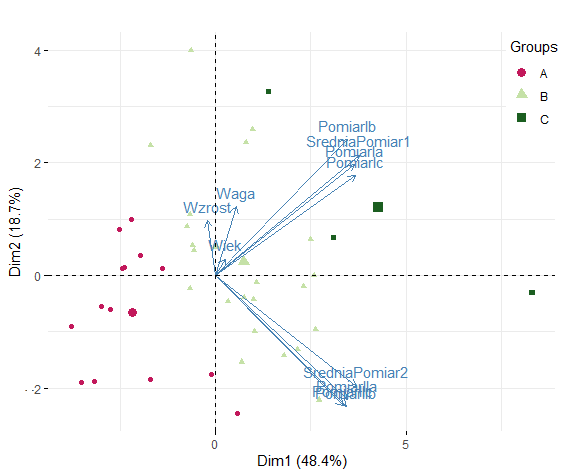
\includegraphics{./Figures/Fig_3.4}
	\caption{Biplot.}
	\label{Fig_3.4}
\end{figure}	




\section{Additional factors}
Impact of air pollution, diet etc.


%----------- Discussion ------------
\chapter{Discussion}
Lorem ipsum dolor sit amet, consetetur sadipscing elitr, sed diam nonumyeirmod tempor invidunt ut labore et dolore magna aliquyam erat, sed diamvoluptua. 


%--------------- Bibliografia ---------------

\begin{thebibliography}{9}
\bibitem{Rosenberg92} Rosenberg M, McCulloch CAG (1992) \emph{Measurement of Oral Malodor: Current Methods and Future Prospects}, Journal of Periodontology, 63, 776–782.
\bibitem{Alasqah16} Alasqah M, Khan S, Elqomsan MA, Gufran K, Kola Z, Bin Hamza MO (2016) \emph{Assessment of halitosis using the organoleptic method and volatile sulfur compounds monitoring}, Journal of Dental Research and Review 3: 3, 94-98.
\bibitem{Lee04} Lee PP, Mak WY, Newsome P (2004) \emph{The aetiology and treatment of oral halitosis: an update}, Hong Kong Medical Journal  10, 414–418.


\bibitem[4]{ }   \emph{ }
\end{thebibliography}


\end{document}